\documentclass[12pt]{article}
\usepackage[utf8]{inputenc}
\usepackage{amssymb,amsmath}
\usepackage{hyperref}
\usepackage{graphicx}
\usepackage{pgf}
\usepackage{tikz}
\input{kvmacros}
\usetikzlibrary{arrows,automata}

\author{Claas Jaehrling, Sven-Hendrik Haase}
\title{RS1 HA zum 16.12.11}
\date{\today}
\begin{document}
\setcounter{secnumdepth}{0}
\maketitle

\section{Aufgabe 8.1}
\subsection{(a)}
\includegraphics{Impulsdiagramm81a}\\
Als Folge von Strukturhazards tritt ein dynamischer 1-Hazard am Ausgang x auf.
\subsection{(b)}
\includegraphics{Impulsdiagramm81b}\\
Als Folge von Strukturhazards tritt ein dynamischer 0-Hazard am Ausgang x auf.
\section{Aufgabe 8.2}
\subsection{(a)}

\subsection{(b)}

\subsection{(c)}

\section{Aufgabe 8.3}
\includegraphics{Impulsdiagramm83a} \\
\includegraphics{Impulsdiagramm83b}

\section{Aufgabe 8.4}
\subsection{(a)}
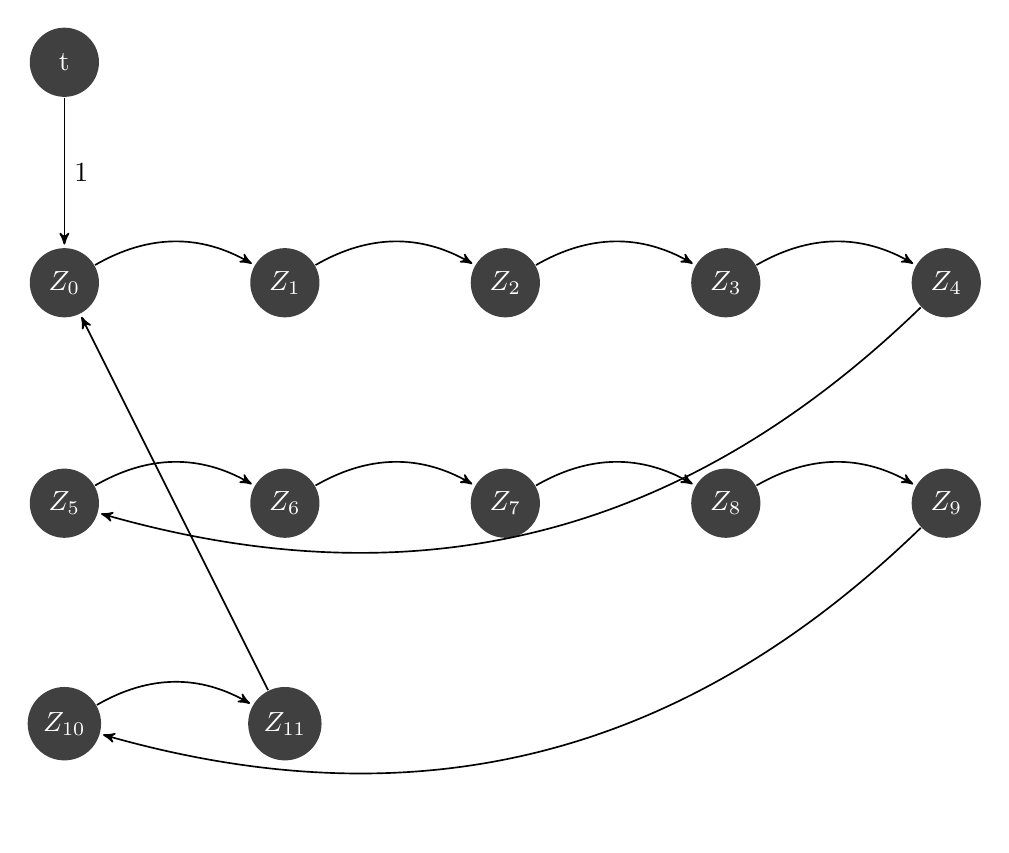
\begin{tikzpicture}[->,>=stealth',shorten >=1pt,auto,node distance=2.8cm,
                    semithick]
  \tikzstyle{every state}=[fill=darkgray,draw=none,text=white]
  
  \node[state]         (t)              {t};
  \node[state]         (A) [below of=t] {\(Z_0\)};
  \node[state]         (B) [right of=A] {\(Z_1\)};
  \node[state]         (C) [right of=B] {\(Z_2\)};
  \node[state]         (D) [right of=C] {\(Z_3\)};
  \node[state]         (E) [right of=D] {\(Z_4\)};
  \node[state]         (F) [below of=A] {\(Z_5\)};
  \node[state]         (G) [right of=F] {\(Z_6\)};
  \node[state]         (H) [right of=G] {\(Z_7\)};
  \node[state]         (I) [right of=H] {\(Z_8\)};
  \node[state]         (J) [right of=I] {\(Z_9\)};
  \node[state]         (K) [below of=F] {\(Z_{10}\)};
  \node[state]         (L) [right of=K] {\(Z_{11}\)};

  \path (t) edge []           node {1} (A)
        (A) edge [bend left]  node {} (B)
        (B) edge [bend left]  node {} (C)
        (C) edge [bend left]  node {} (D)
        (D) edge [bend left]  node {} (E)
        (E) edge [bend left]  node {} (F)
        (F) edge [bend left]  node {} (G)
        (G) edge [bend left]  node {} (H)
        (H) edge [bend left]  node {} (I)
        (I) edge [bend left]  node {} (J)
        (J) edge [bend left]  node {} (K)
        (K) edge [bend left]  node {} (L)
        (L) edge []           node {} (A);
\end{tikzpicture}

\subsection{(b)}
\begin{tabular}{c|c c c c||c c c c|c c c|c c}
t & \(z_3\) & \(z_2\) & \(z_1\) & \(z_0\) & \(z_3^+\) & \(z_2^+\) &
    \(z_1^+\) & \(z_0^+\) & \(rt_A\) & \(ge_A\) & \(gr_A\) & \(rt_F\)
    & \(gr_F\) \\
\hline
% t   z3  z2  z1  z0  z3+ z2+ z1+ z0+ rtA geA grA rtF grF
  0 & 0 & 0 & 0 & 0 & 0 & 0 & 0 & 0 & 0 & 0 & 1 & 1 & 0 \\
  1 & 0 & 0 & 0 & 0 & 0 & 0 & 0 & 1 & 0 & 0 & 1 & 1 & 0 \\
  * & 0 & 0 & 0 & 1 & 0 & 0 & 1 & 0 & 0 & 1 & 0 & 1 & 0 \\
  * & 0 & 0 & 1 & 0 & 0 & 0 & 1 & 1 & 1 & 0 & 0 & 1 & 0 \\
  * & 0 & 0 & 1 & 1 & 0 & 1 & 0 & 0 & 1 & 0 & 0 & 0 & 1 \\
  * & 0 & 1 & 0 & 0 & 0 & 1 & 0 & 1 & 1 & 0 & 0 & 0 & 1 \\
  * & 0 & 1 & 0 & 1 & 0 & 1 & 1 & 0 & 1 & 0 & 0 & 0 & 1 \\
  * & 0 & 1 & 1 & 0 & 0 & 1 & 1 & 1 & 1 & 0 & 0 & 0 & 1 \\
  * & 0 & 1 & 1 & 1 & 1 & 0 & 0 & 0 & 1 & 0 & 0 & 1 & 0 \\
  * & 1 & 0 & 0 & 0 & 1 & 0 & 0 & 1 & 1 & 1 & 0 & 1 & 0 \\
  * & 1 & 0 & 0 & 1 & 1 & 0 & 1 & 0 & 0 & 0 & 1 & 1 & 0 \\
  * & 1 & 0 & 1 & 0 & 1 & 0 & 1 & 1 & 0 & 0 & 1 & 1 & 0 \\
  * & 1 & 0 & 1 & 1 & 1 & 1 & 0 & 0 & 0 & 0 & 1 & 1 & 0 \\
  * & 1 & 1 & 0 & 0 & 1 & 1 & 0 & 1 & 0 & 0 & 1 & 1 & 0 \\
  * & 1 & 1 & 0 & 1 & 1 & 1 & 1 & 0 & 0 & 0 & 0 & 0 & 0 \\
  * & 1 & 1 & 1 & 0 & 1 & 1 & 1 & 1 & 0 & 0 & 0 & 0 & 0 \\
  * & 1 & 1 & 1 & 1 & 0 & 0 & 0 & 0 & 0 & 0 & 0 & 0 & 0 \\
\end{tabular}
  
\subsection{(c)}
%\[z_3^+\]
%\karnaughmap{4}{f(\(z_3^+\),\(z_2^+\),\(z_1^+\),\(z_0^+\)):}{{\(z_3^+\)}{\(z_2^+\)}{\(z_1^+\)}{\(z_0^+\)}}{0000000011111111}{}

\subsection{(d)}
\begin{tikzpicture}[->,>=stealth',shorten >=1pt,auto,node distance=2.8cm,
                    semithick]
  \tikzstyle{every state}=[fill=darkgray,draw=none,text=white]
  
  \node[state]         (M) [right of=t] {\(Z_{12}\)};
  \node[state]         (N) [right of=M] {\(Z_{13}\)};
  \node[state]         (O) [right of=N] {\(Z_{14}\)};
  \node[state]         (P) [right of=O] {\(Z_{15}\)};
  \node[state]         (A) [below of=t] {\(Z_0\)};
  \node[state]         (B) [right of=A] {\(Z_1\)};
  \node[state]         (C) [right of=B] {\(Z_2\)};
  \node[state]         (D) [right of=C] {\(Z_3\)};
  \node[state]         (E) [right of=D] {\(Z_4\)};
  \node[state]         (F) [below of=A] {\(Z_5\)};
  \node[state]         (G) [right of=F] {\(Z_6\)};
  \node[state]         (H) [right of=G] {\(Z_7\)};
  \node[state]         (I) [right of=H] {\(Z_8\)};
  \node[state]         (J) [right of=I] {\(Z_9\)};
  \node[state]         (K) [below of=F] {\(Z_{10}\)};
  \node[state]         (L) [right of=K] {\(Z_{11}\)};

  \path
        (A) edge [bend left]  node {t=0} (M)
        (M) edge [bend left]  node {t=0} (N)
        (N) edge [bend left]  node {t=0} (O)
        (O) edge [bend left]  node {t=0} (P)
        (M) edge []  node {t=1} (B)
        (N) edge []  node {t=1} (B)
        (O) edge []  node {t=1} (B)
        (P) edge []  node {t=1} (B)
        (P) edge [loop]  node {t=0} (P)
        (A) edge [bend left]  node {t=1} (B)
        (B) edge [bend left]  node {} (C)
        (C) edge [bend left]  node {} (D)
        (D) edge [bend left]  node {} (E)
        (E) edge [bend left]  node {} (F)
        (F) edge [bend left]  node {} (G)
        (G) edge [bend left]  node {} (H)
        (H) edge [bend left]  node {} (I)
        (I) edge [bend left]  node {} (J)
        (J) edge [bend left]  node {} (K)
        (K) edge [bend left]  node {} (L)
        (L) edge []           node {} (A);
\end{tikzpicture}

\end{document}
